\documentclass{article}

% Language setting
% Replace `english' with e.g. `spanish' to change the document language
\usepackage[english]{babel}

% Set page size and margins
% Replace `a4paper' with `letterpaper' for US standard size
\usepackage[a4paper,top=2cm,bottom=2cm,left=3cm,right=3cm,marginparwidth=1.75cm]{geometry}

% Useful packages
\usepackage{amsmath}
\usepackage{graphicx}
\usepackage[colorlinks=true, allcolors=blue]{hyperref}
\usepackage{natbib} %bibliography
\usepackage{tabularx} %tables
\usepackage{longtable} %also tables
\usepackage{caption} % Changing caption font in tables and figures
\usepackage{enumerate} %for enumeration
\usepackage{array} %to create modifications to the tables
\usepackage{float} %figures and captions
\usepackage{mathtools}
\usepackage{subcaption} %  for subfigures environments 


\title{Predicting the Adoption Curve of a New Technology Using Helium Hotpots as a Case Study.}
\author{Ciupitu, Octavian; Talantceva, Marina}

%------------------------------------------------
% Document Starts Here
%------------------------------------------------
\begin{document}

\date{\today}
\maketitle

\begin{center}
    Predicting the adoption curve of Helium Hotspotsusing the Bass Model \citep{bass1969new}.
\end{center}
  
%------------------------------------------------
% CHAPTER 1
%------------------------------------------------

\section{The Bass Model}

The \emph{Bass Model} was originated by Frank Bass in 1969 and is used to predict new product diffusion patterns. In his first paper
in 1969, Bass built on the findings of \cite{rogers2014diffusion} on the \emph{Diffusion of Innovations}, which were first pubished in 1963,
and introduced what he called a \emph{new product growth model for consumer durables}. Later, this model proved to be applicable to more
products than just consumer durables, and eventually became worldwide known as the \emph{Bass Model}. The model is used to explain the
interaction between current and potential adopters of a new product. It states that there are two types of adopters - \emph{innovators} and
\emph{imitators}. This means, the speed and timing of adoption depends on the degree of innovation and the degree of imitation among adopters.
Accoding to Bass, these are the two main kinds of forces determining the diffusion pattern.

\medskip

\noindent There are three key parameters in the Bass Model - usually called $p$, $q$, and $m$:

\begin{enumerate}
    \item $p$ is called the \emph{coefficient of innovation} and represents the rate or probability that an innovator will adopt at time t. 
    \item $q$ is called the \emph{coefficient of imitation} and accounts for the “word of mouth” or “social contagion” effects.
    \item $m$ indicates the market size and provides the scale of the demand forecast. Unlike the other two parameters $p$ and $q$,
    $m$ does not determine the shape of the adoption curve. 
\end{enumerate}

\begin{figure}[hptb]
    \centering{}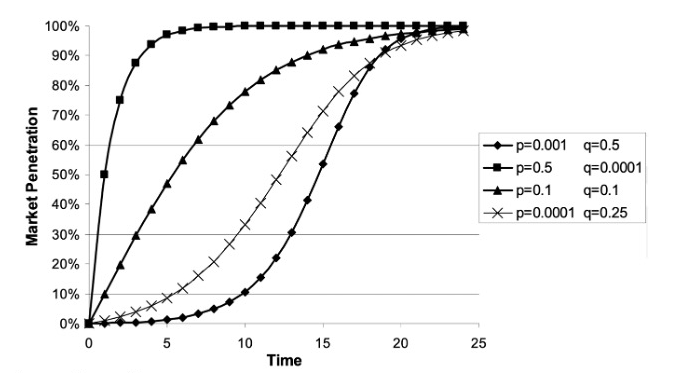
\includegraphics[scale=0.45]{plots/bass_model_example.png}\\
    \caption{Based on Number Analytics (2021).}
\end{figure}

\noindent At the beginning of a product diffusion process, the \emph{coefficient of innovation} is particularly important, as it represents the set of
people who are the first to adopt the new product regardless of the actions of others - in other words, they are \emph{innovators}. Later in the diffusion
process, the \emph{coefficient of imitation} becomes more and more important. It stands for the set of people who adopt due to the fact that they see
products on other people. The \emph{coefficient of imitation} represents the contagion effect in a population and describes the influence of the \emph{imitators}.

\medskip

\noindent The two parameters $p$, and $q$ specify how fast or slow the adoption of a new product is expected to proceed. To sum up, the adoption of a
new product can proceed either by small scale or a large scale (specified by $m$) or at a fast or slow pace (specified by $p$ and $q$). 
Figure 1 shows different estimated curves with various levels of innovation ($p$) and imitation ($q$). The level of $p$ determines the adoption rate at
the beginning of the diffusion process, whereas the level of $q$ determines the adoption rate at the time where many adoptions have already taken place.
Characteristic of these diffusion curves is their S-shape, which illustrates that the adoption rate of a new product is particularly low at the beginning,
when no contagion effects can yet exist, and at the end, when market saturation has been reached. 

\medskip

\noindent We derive the estimation function from the Bass equation below:

\begin{equation} \label{eq1}
    \begin{split}
        \frac{f(t)}{m - F(t)} = p + q * \frac{F(t)}{m}\\
    \end{split}
\end{equation}

\noindent Where $F(t)$ is the installed base fraction, i.e. the number of current cumulative adoptions; $f(t)$ is the change of the installed base
fraction, i.e. the number of new adoptions in a specific timeframe; $p$ is the coefficient of innovation; and $q$ is the coefficient of imitation.
In order to estimate those parameters, an estimation funciton needs to be derived. Using some simple algebra we get:

\begin{equation} \label{eq2}
    \begin{split}
    f(t) & = \left[ p + \frac{q * F(t)}{m} \right] * (m - F(t)) \\
    \end{split}
\end{equation}

\begin{equation} \label{eq3}
    \begin{split}
    f(t) & = a + b * N(t) + c * \left[ N(t) \right]^2
    \end{split}
\end{equation}

\noindent Where we can derive that:

\begin{equation}
    \begin{aligned}
    a & = p*m \\[2pt]
    b & = q - p \\[2pt]
    c & = - \frac{q}{m} \\[15pt]
    m & = \frac{-b \pm \sqrt{b^2 -4ac}}{2c} \\
    p & = \frac{a}{m} \\[2pt]
    q & = -m*c
    \end{aligned}
\end{equation}

\bigskip

\noindent Using the estimation function from \emph{Equation 3}, a linear regression can be performed. The resulting parameters $a$, $b$ and $c$ can be
then used to calculate the coefficient of innovation $p$, the coefficient of imitation $q$ and the market size $m$ by applying the formulas from \emph{Equation 4}.

\clearpage

%------------------------------------------------
% CHAPTER 2
%------------------------------------------------

\section{Data Analysis and Results}

As a first step, we collect all hostpot adoptions from the Helium blockchain for New York City, US. We consider New York as an interesting study
environment since it is a comparatively fast adopting city. The installation date of a hotspot is stored in the blockchain by a daily frequency. However, to
avoid many zero entries in our dataset, especially at the beginning of the hotspot diffusion process, we decided to transform our dataset to a weekly frequency.
This allows us to observe the evolution of adoptions from week to week, as can be seen in the left chart of Figure 2 (weekly adoptions) as well as on the right
one (weekly cumulative adoptions).

\begin{figure}[!hptb]
    \begin{subfigure}[h]{0.52\linewidth}
    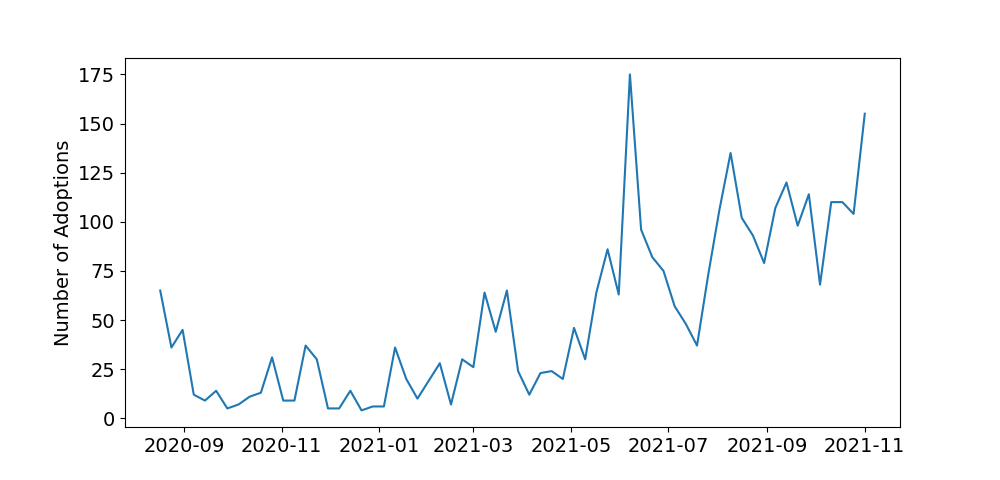
\includegraphics[width=\linewidth]{plots/weekly_hotspot_adoptions.png}
    \end{subfigure}
    \hfill
    \begin{subfigure}[h]{0.52\linewidth}
    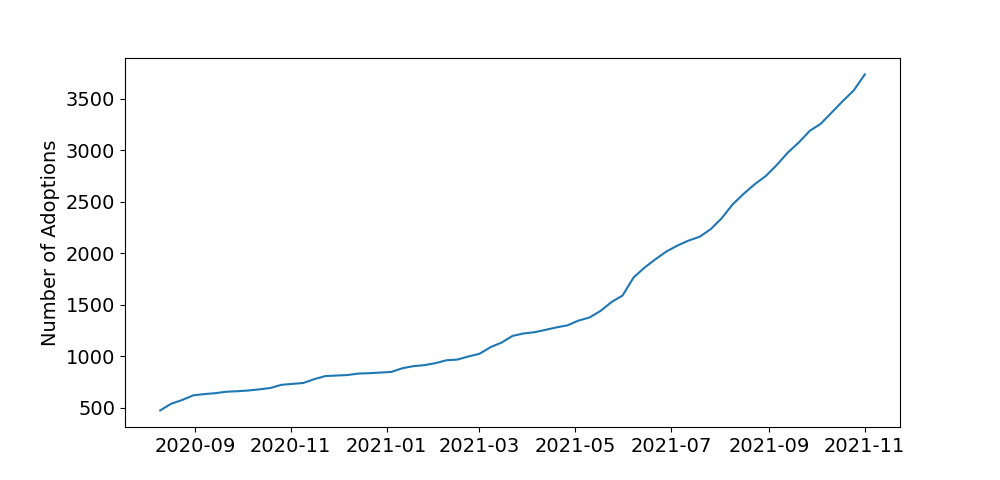
\includegraphics[width=\linewidth]{plots/weekly_hotspot_adoptions_cumulative.png}
    \end{subfigure}%
    \caption{Number of weekly new adoptions (left) and weekly cumulative hotspot adoptions (right).}
    \end{figure}


\noindent Especially in Figure 2 (right), it can be clearly seen that the number of adoptions is still increasing rapidly and saturation has not been reached yet.
So it is very interesting to fit the Bass Model based on this data set to predict the next period. We examine the period from August 10, 2020 to November 7, 2021,
which corresponds to an observation period of 65 weeks. We then use the estimated Bass Model based on this period to predict the evolution of adoption numbers until
the end of 2022, more precisely until December 26, 2022.

\bigskip

\noindent The estimates of our analysis give us a coefficient of innovation $p$ of $0.00066$, a coefficient of imitation $q$ of $0.055$, and a market size $m$ of $9754$. If we
plot our fitted curve against actual weekly (new) hotspot adoptions as in Figure 3, we can see that the fitted curve describes reality well.

\begin{figure}[!hptb]
    \centering{}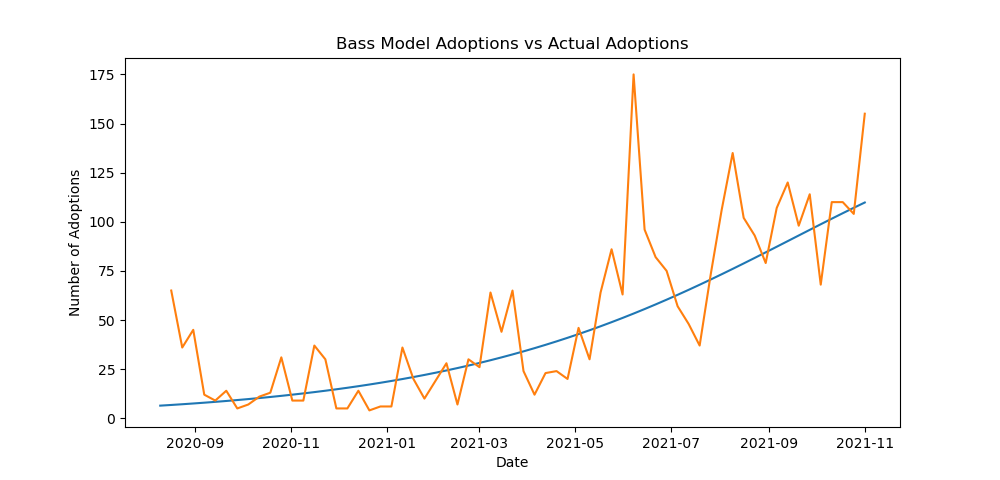
\includegraphics[scale=0.6]{plots/bass_model_adoptions_vs_actual_adoptions.png}\\
    \caption{Fitted Bass Model (blue) vs. Actual Hotspots Adoptions from the Training Dataset (orange).}
\end{figure}

\noindent Figure 4 again shows, similar to Figure 3, our fitted curve, but this time against the weekly cumulative hotspot adoptions. Additionally, we inclueded the prediction
of our Bass Model until the end of 2022. It can be seen that, according to our prediction, the saturation will be reached at the beginning of 2023 at around $9,700$ adoptions,
just as our estimated parameter $m$ suggested.

\bigskip
\bigskip
\bigskip
\bigskip

\begin{figure}[!hptb]
    \centering{}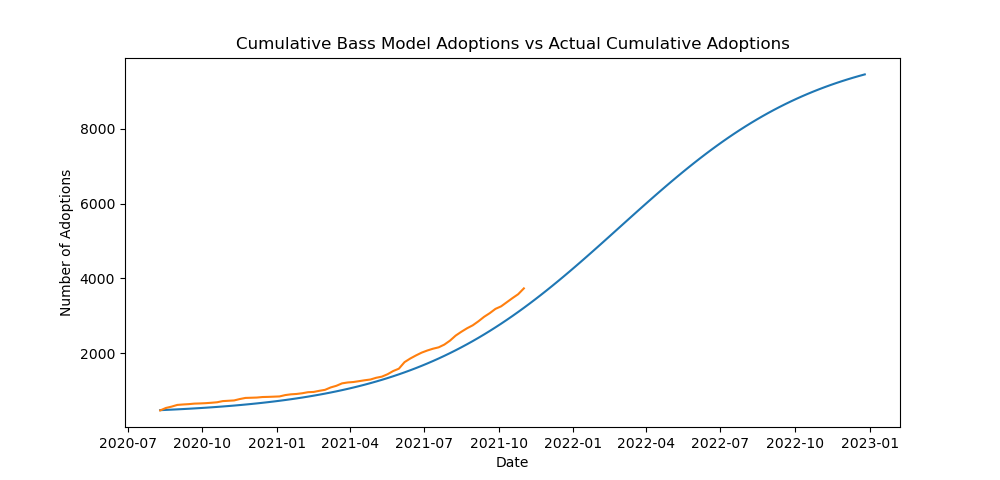
\includegraphics[scale=0.6]{plots/cumulative_bass_model_adoptions_vs_actual_cumulative_adoptions.png}\\
    \caption{Bass Model Estimation until the End of 2022 (blue) vs. Actual Adoption until November 2021 (orange).}
\end{figure}

\noindent In a final step, we compare the Bass Model prediction with the real hotspots adoptions until December 2022. The result can be seen in Figure 5. It can be seen, that our
prediction is clearly too optimisitc and that the actual market saturation is reached at around $6000$ hotspots.

\begin{figure}[!hptb]
    \centering{}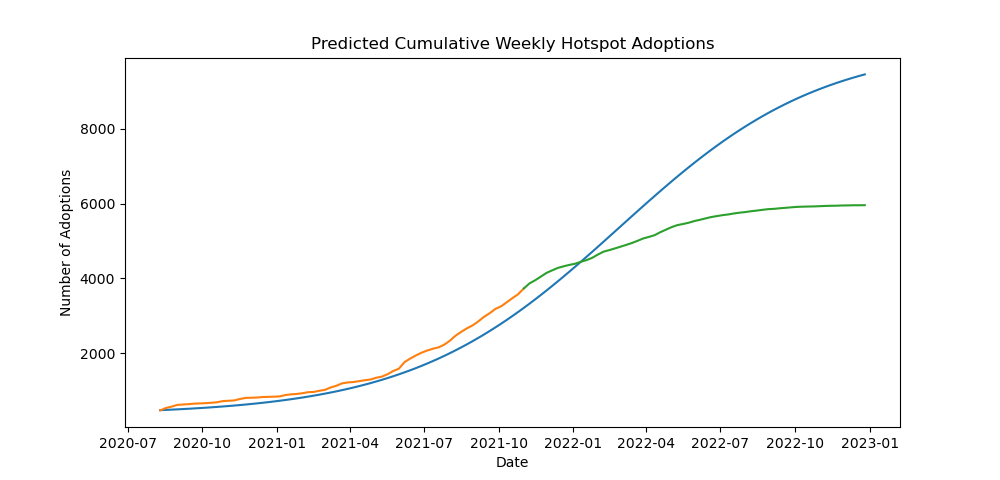
\includegraphics[scale=0.6]{plots/predicted_cumulative_weekly_hotspot_adoptions.png}\\
    \caption{Bass Model Estimation until the End of 2022 (blue) vs. Actual Adoption until the End of 2022 (orange + green).}
\end{figure}

%------------------------------------------------
% CHAPTER 3
%------------------------------------------------

\section{Discussion and Limitations}

Our analysis clearly shows that our prediction is too optimistic when compared to the test data set. The market size estimated by the Bass Model is $m = 9,754$, whereas
from the real data we can see that the hotspot adoptions tend to converge towards a market size of $6000$. However, a closer look at the model quickly reveals where
this discrepancy comes from. The Bass model, which is now over 50 years old, is one of the first models to describe the diffusion process of a new product, and is
therefore still very simply designed. Namely, it describes the dependent variable only on the basis of its own lags i.e. the so-called "installed base". For a more
complex technology, like in our case a Helium hotspot, estimating future adoptions solely based on past adoptions does not seem to be sufficient for a good fit.
The reason for this is that a potential consumer's adoption decision depends on additional important market variables. Probably the most important market variable
is the performance of the cryptocurrency market, or to be more precise, the so-called Helium Token (\$HNT), which rewards consumers for setting up and operating a
hotspot. If the price of \$HNT, which can be traded for traditional currencies such as dollars or euros on crypto exchanges, is high, then consumers'
incentives to adopt also increase. 

\bigskip

\noindent However, if we look at the past performance of the cryptocurrency market, we see that for the period of our training data set (August 10, 2020 to November 7, 2021) all
cryptocurrencies massively increase in value. Not only did the price of the Helium Token reach its peak at around \$52 in November 2021, but also the price of other major
cryptocurrencies like Bitcoin or Ethereum. This means, that the estimation of our variables $p$, $q$ and $m$ is based on a timeframe when the whole market was going up. However,
shortly after the end of our training data set the cryptocurrency market crashed in 2022, causing a lot of currencies to loose up to 80\% of their market capitalization. This in
turn caused less people to adopt Helium hotspots since the incentives for doing so went down. This fact is also well illustrated by Figure 6. Here it can be clearly seen that the
rate of new adoptions drops rapidly as soon as the HNT price collapses (around February 2022). The collapse of the HNT price is an essential piece of information that our model
does not take into account.

\begin{figure}[!hptb]
    \centering{}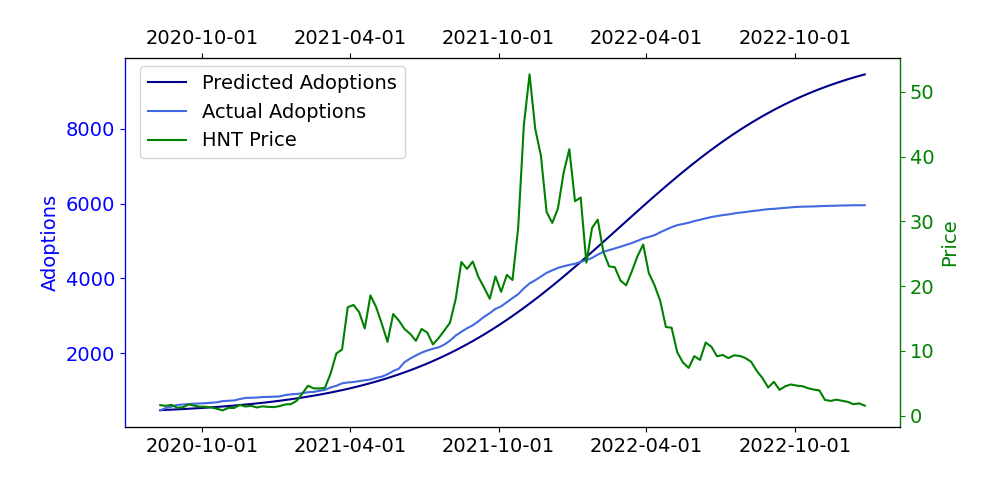
\includegraphics[scale=0.6]{plots/hnt_comparison.png}\\
    \caption{The Decline in Hotspot Adoptions after HNT Price Collapse.}
\end{figure}

\noindent To account for additional variables, Frank Bass years later presented an extension of his original model that captures the influence of such external variables with the
publication of the \emph{Generalized Bass Model} \citep{bass1994bass}. For future research, we therefore propose to use the \emph{Generalized Bass Model} both to gain better
predictions about the diffusion process and to gain accurate insights into which external variables have an impact on the adoption rate, i.e., on the slope of the adoption curve.


%%%%%%%%%%%%%%%%%% REFERENCES %%%%%%%%%%%%%%%%%%%%%%%%
\setcounter{secnumdepth}{0}
\addcontentsline{toc}{section}{References}
\bibliographystyle{chicago}
\bibliography{Biblio.bib} 
%%%%%%%%%%%%%%%%%%%%%%%%%%%%%%%%%%%%%%%%%%%%%%%%%%%%%%%%
 
\end{document}